\documentclass[
	12pt,twoside,a4paper
]{report}

\usepackage{graphicx}
\usepackage[margin=1in]{geometry}
\usepackage{fancyhdr}
\usepackage[utf8]{inputenc}
\usepackage{etoc}
\usepackage{xcolor, soul}
\usepackage{listings}
\usepackage{amsmath}
\usepackage{lipsum}
\usepackage{pgfplots}
\usepackage{hyperref}
\usepackage{circuitikz}
\usepackage{caption}
\usepackage{subcaption}
\usepackage[style=apa, backend=biber]{biblatex}

\addbibresource{refs.bib}
\DeclareLanguageMapping{english}{english-apa}

\sethlcolor{yellow}

\fancypagestyle{plain}{
	\fancyhf{}
	\fancyhead[l]{Project 1}
	\fancyhead[r]{April 26, 2024}
	\fancyfoot[le, ro]{Page \thepage}
	\fancyfoot[re, lo]{ESD Capsule 2024}
	\setlength{\headheight}{15pt}
	\renewcommand{\headrulewidth}{0.2pt}
	\renewcommand{\footrulewidth}{0.2pt}
}	

\thispagestyle{plain}

\renewcommand{\etocaftertitlehook}{\thispagestyle{plain}}
\renewcommand{\etocaftertochook}{\thispagestyle{plain}}

\begin{document}
	\begin{center}
	\includegraphics[width=0.4\textwidth]{assets/agu.png}

	\Huge
	\textbf{Project \#1}

	\vspace{0.3cm}
	\Huge
	Capacitor Design \& Measurement

	\vspace{0.8cm}
	\large
	\vspace{0.5cm}
	\LARGE
	\vspace{1.5cm}
	\textbf{}
	\vfill
	\vspace{0.8cm}
	\Large
\end{center}

\begin{tabbing}
	\hspace*{1em} \= \hspace*{8em} \= \hspace*{11em} \= \kill
	\> Barış DEMİRCİ \> agu@338.rocks \> \\
	\> \> \> \\
	\>  April 26, 2024 \> \> \\
\end{tabbing}

	\tableofcontents

	\chapter{Introduction}
In this project, we designed and constructed two types of capacitors: a parallel-plate capacitor and a cylindrical capacitor. We then designed experiments to measure the capacitance of these capacitors and compared the results with theoretical calculations. Additionally, we investigated the behavior of capacitors in circuits, including their response to triangular wave input and their charge dynamics in series circuits. Also learned how to effectively use oscilloscope and function generator to measure the voltage and current in the circuits.

	\chapter{Capacitor Design}

\section{Parallel Plate Capacitor}

We have made a simple $200mm\times150mm\times5mm$ design on SolidWorks and 3D printed the model with 2 different settings. The first model was printed with 75\% infill and the second model was printed with 15\% infill. The 3D printed model \& design are shown in Figure \ref{fig:3d-printed-models}.

\begin{figure}[h]
    \centering
    \includegraphics[width=0.9\linewidth]{assets/parallel-plate-design.png}
    \caption{3D Printed Model \& Design}
    \label{fig:3d-printed-models}
\end{figure}

We have covered the 3D printed model with aluminum foil to get a parallel plate capacitor.

\newpage
\thispagestyle{plain}

\section{Cylindirical Capacitor}
For cylindirical capacitor, we get 2 steel pipe one with 30mm diameter and 22cm length and the other with 40mm diameter and 22cm length. We have designed a lock mechanism to connect the pipes and make them a cylindirical capacitor. The design is shown in Figure \ref{fig:cylindirical-design}.

\begin{figure}[h]
    \centering
    \includegraphics[width=0.9\linewidth]{assets/cylindirical-design.png}
    \caption{Cylindirical Capacitor Design}
    \label{fig:cylindirical-design}
\end{figure}

To change the capacitance of the capacitor, we have designed a sliding mechanism to change the distance between the plates.

	\chapter{Measuring Capacitance}

In order to measure the capacitance of the capacitors without using the "capacitance" function on the digital multimeter, we have used the circuit shown in Figure \ref{fig:capacitance-circuit}:

\begin{figure}[h]
    \centering
    \begin{circuitikz} \draw
        (0,0) to[square voltage source, l=0-5V] (0,4)
        to[R, l=$5k\Omega$] (4,4) 
        to[C, l=C] (4,0) -- (0,0)
        ;
        \end{circuitikz}
    \caption{Circuit to Measure Capacitance}
    \label{fig:capacitance-circuit}
\end{figure}

The circuit consists of a square wave voltage source @ 5V zero-to-peak, a 5k$\Omega$ resistor and a capacitor. The voltage across the capacitor is measured using the oscilloscope. The time taken for the voltage to reach 63.2\% of the maximum voltage is measured. The capacitance is then calculated using the formula:

\begin{align*}
    &V(t) = V_{\max} \cdot e^{-\frac{t}{RC}} \\
    &\boxed{C = \frac{t}{R}}
\end{align*}

Where:
\begin{itemize}
    \item C is the capacitance in Farads
    \item t is the time taken for the voltage to reach 63.2\% of the maximum voltage in seconds
    \item R is the resistance in Ohms
\end{itemize}

\newpage
\thispagestyle{plain}

\section{Theoretical Analysis}
We have decided to use this circuit to measure the capacitance of the capacitors. The circuit is shown in Figure \ref{fig:capacitance-circuit}. First, we tested if the circuit is working by trying everything in LTSpice:

\begin{figure}[h]
    \centering
    \includegraphics[width=0.8\textwidth]{assets/1714061123.png}
    \caption{LTSpice Simulation of the Circuit}
    \label{fig:ltspice-simulation}
\end{figure}

We have theoretically calculated the capacitance of our capacitor and compared the results from the simulation and the theoretical calculations.


\begin{table}[h]
    \centering
    \begin{tabular}{l|l|l|}
    \cline{2-3}
                                                            & $\epsilon_r$ & Theoretical Capacitance \\ \hline
    \multicolumn{1}{|l|}{PLA \textbackslash{}w 75\% Infill} & 2.4     & 1.3nF                       \\ \hline
    \multicolumn{1}{|l|}{PLA \textbackslash{}w 15\% Infill} & 0.48    & 0.26nF                \\ \hline
    \multicolumn{1}{|l|}{Cylindirical} & 1 (Empty)    & 43pF                  \\ \hline
    \end{tabular}
    \caption{Theoretical Capacitance Values}
\end{table}

And after checking the results from the simulation, we have seen that the results are very close to the theoretical calculations ($\pm10\%$). Therefore, we have decided to use this circuit to measure the capacitance of the capacitors.


\newpage{}
\thispagestyle{plain}

\section{Results}

We have measured the time taken for the voltage to reach 63.2\% of the maximum voltage using the oscilloscope because after $RC$ seconds later the voltage reachs this value. Table \ref{fig:time-taken} shows the time taken for the voltage to reach 63.2\% of the maximum voltage for the capacitors:

\begin{center}
    \begin{table}[h]
        \centering
            \begin{tabular}{l|l|l|l|}
            \cline{2-4}
                                    & Cylindirical & Parallel \textbackslash{}w 75\% Infill & Parallel \textbackslash{}w 15\% Infill \\ \hline
            \multicolumn{1}{|l|}{t} & $200\mu s$          & $7ms$                                   & $2ms$                                     \\ \hline
            \end{tabular}
        \caption{Time Taken for Voltage to Reach 63.2\% of Maximum Voltage}
        \label{fig:time-taken}
        \end{table}
\end{center}

The resistance used in the circuit is 5k$\Omega$. Using the formula mentioned above, the capacitance of the capacitors is calculated as follows:

\begin{align*}
    C_{cylindrical} &= \frac{200\mu s}{5k\Omega} = \boxed{40pF} \\
    C_{parallel~75\%~Infill} &= \frac{7ms}{5k\Omega} = \boxed{1.4nF} \\
    C_{parallel~15\%~Infill} &= \frac{2ms}{5k\Omega} = \boxed{0.4nF}
\end{align*}

\section{Comparing Simulation \& Measurement Results}

The capacitance of the capacitors is calculated using circuit shown in Figure \ref{fig:capacitance-circuit} and the formula mentioned above. We have set the circuit up and measured time values of the capacitors:

\begin{figure}[h]
    \centering
    \includegraphics[width=0.6\textwidth]{assets/2WhatsApp Image 2024-04-18 at 20.32.11.jpeg}
    \caption{Circuit Setup}
    \label{fig:circuit-setup}
\end{figure}

\newpage
\thispagestyle{plain}

We can easily see the charging and discharging of the capacitor in the oscilloscope:

\begin{figure}[h]
    \centering
    \includegraphics[width=0.6\textwidth]{assets/WhatsApp Image 2024-04-16 at 18.20.12 (2).jpeg}
    \caption{Oscilloscope Results}
    \label{fig:oscilloscope-results}
\end{figure}

The same circuit is simulated using LTSpice. The simulation results are shown in Figure \ref{fig:ltspice-simulation}:

\begin{figure}[h]
    \centering
    \includegraphics[width=0.8\textwidth]{assets/1714059734.png}
    \caption{LTSpice Simulation Results}
    \label{fig:ltspice-simulation}
\end{figure}

We can easily see the charging and discharging of the capacitor in the simulation results. 

If we compare the simulation and the measurement results, we can see that the results are very close to each other. The capacitance values are calculated as follows:

\begin{table}[h]
    \centering
    \begin{tabular}{l|l|l|}
    \cline{2-3}
                                                            & Simulation & Measurement \\ \hline
    \multicolumn{1}{|l|}{PLA \textbackslash{}w 75\% Infill} & 1.3nF     & 1.4nF      \\ \hline
    \multicolumn{1}{|l|}{PLA \textbackslash{}w 15\% Infill} & 0.26nF    & 0.4nF      \\ \hline
    \multicolumn{1}{|l|}{Cylindirical} & 43pF     & 40pF       \\ \hline
    \end{tabular}
    \caption{Simulation \& Measurement Results}
\end{table}



\newpage
\thispagestyle{plain}

\section{Variation of Capacitance}

Our designed capacitors are variable capacitors and their capacitance values can be changed. 

\subsection{Parallel Plate Capacitors}

For parallel plate capacitor, we can calculate the capacitance with the following equation:

\begin{align*}
    C &= \varepsilon\cdot\frac{A}{d}
\end{align*}

Where:
\begin{itemize}
    \item C is the capacitance in Farads
    \item $\varepsilon$ is the permittivity of the dielectric material in Farads per meter ($\varepsilon_0\varepsilon_r$)
    \item A is the area of the plates in square meters
    \item d is the separation between the plates in meters
\end{itemize}

The capacitance of the parallel plate capacitor can be changed by changing any value in the equation. We have decided to change $\varepsilon~(=\varepsilon_0\cdot\boxed{\varepsilon_r})$ value by varying the infill density of the plates.
The capacitance of the parallel plate capacitor is directly proportional to the permittivity of the dielectric material. The capacitance of the capacitor with 75\% infill density is higher because the permittivity of the dielectric material is higher. 

\begin{figure}[h]
    \centering
    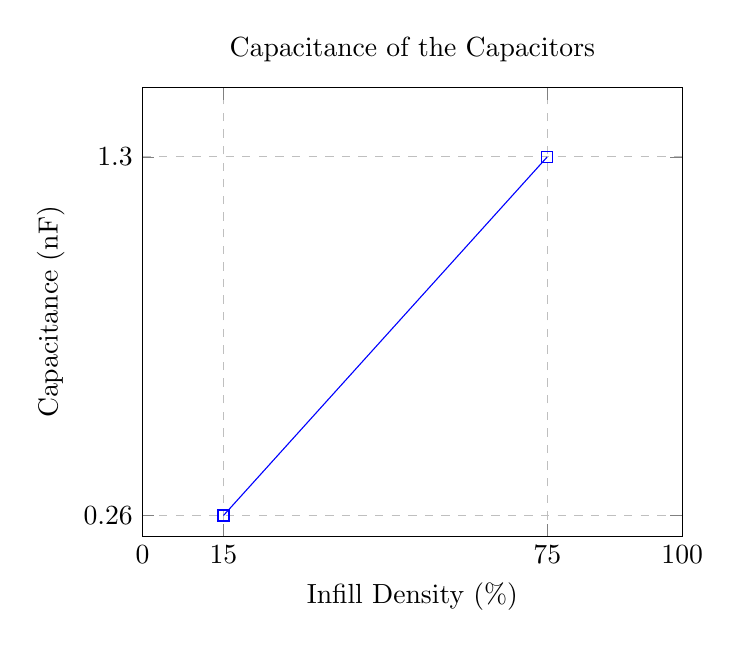
\begin{tikzpicture}
        \begin{axis}[
            title={Capacitance of the Capacitors},
            xlabel={Infill Density (\%)},
            ylabel={Capacitance (nF)},
            xmin=0, xmax=1,
            ymin=0.2, ymax=1.5,
            xtick={0, 0.15, 0.75, 1},
            ytick={0, 0.26, 1.3},
            xticklabels={0, 15, 75, 100},
            yticklabels={0, 0.26, 1.3},
            legend pos=north west,
            ymajorgrids=true,
            xmajorgrids=true,
            grid style=dashed,
        ]
        
        \addplot[
            color=blue,
            mark=square,
            ]
            coordinates {
            (0.15, 0.26)
            (0.75, 1.3)
            };
        
        \end{axis}
    \end{tikzpicture}
    \caption{Capacitance vs Infill Density Table}
    \label{fig:capacitance-plot}
\end{figure}

\newpage
\thispagestyle{plain}

\subsection{Cylindrical Capacitors}

For cylindrical capacitor, we can calculate the capacitance with the following equation:

\begin{align*}
    C &= 2\pi\varepsilon\frac{L}{\ln{\frac{r_2}{r_1}}}
\end{align*}

Where:
\begin{itemize}
    \item C is the capacitance in Farads
    \item $\varepsilon$ is the permittivity of the dielectric material in Farads per meter ($\varepsilon_0\varepsilon_r$)
    \item L is the length of the cylinder in meters
    \item $r_1$ is the inner radius of the cylinder in meters
    \item $r_2$ is the outer radius of the cylinder in meters
\end{itemize}

The capacitance of the cylindrical capacitor can be changed by changing any value in the equation. We have decided to change $L$ value by varying the height of the cylinder as shown in Figure \ref{fig:cylindirical-varying}. The capacitance of the cylindirical capacitor is directly proportional to length of the capacitor. The capacitance of the capacitor with 22cm height is higher than with 10cm height because the length of the capacitor is higher.

\begin{figure}[h]
    \centering
    \includegraphics[width=1\textwidth]{assets/cylindirical-variable.png}
    \caption{Cylindirical Capacitor Varying}
    \label{fig:cylindirical-varying}
\end{figure}

\newpage
\thispagestyle{plain}

We have made 5 different measurements for the cylindrical capacitor. Calculated the capacitance values using the same formula mentioned above ($C = \frac{t}{R}$). The capacitance values are shown in Figure \ref{fig:cylindirical-capacitance-plot}:

\begin{figure}[h]
    \centering
    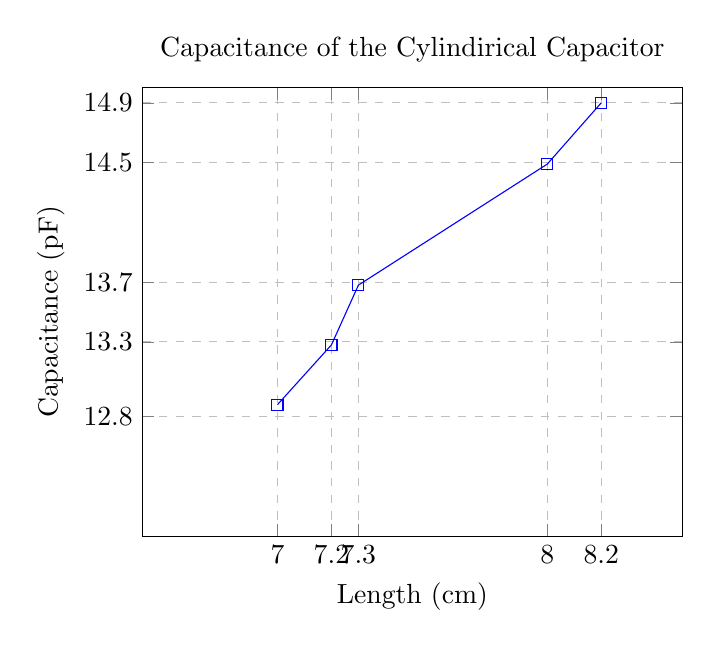
\begin{tikzpicture}
        \begin{axis}[
            title={Capacitance of the Cylindirical Capacitor},
            xlabel={Length (cm)},
            ylabel={Capacitance (pF)},
            xmin=6.5, xmax=8.5,
            ymin=12, ymax=15,
            legend pos=north west,
            ymajorgrids=true,
            xmajorgrids=true,
            grid style=dashed,
            xtick={7, 7.2, 7.3, 8, 8.2},
            ytick={12.8, 13.3, 13.7, 14.5, 14.9},
        ]
        
        \addplot[
            color=blue,
            mark=square,
            ]
            coordinates {
            (7, 12.88)
            (7.2, 13.28)
            (7.3, 13.68)
            (8, 14.49)
            (8.2, 14.9)
            };
        
        \end{axis}
    \end{tikzpicture}
    \caption{Capacitance vs Length Table}
    \label{fig:cylindirical-capacitance-plot}
\end{figure}

	\chapter{Using Capacitors}

We have connected out capacitor to a triangular voltage source and a resistor. The circuit is shown in Figure \ref{fig:triangular-circuit}.

\begin{figure}[h]
    \centering
    \begin{circuitikz} \draw
        (0,0) to[triangle voltage source] (0,4)
        to[R, l=$5k\Omega$] (4,4) 
        to[C, l=C] (4,0) -- (0,0)
        ;
        \end{circuitikz}
    \caption{Circuit with Triangular Voltage Source \& Capacitor}
    \label{fig:triangular-circuit}
\end{figure}

The voltage source is a triangular wave with a peak-to-peak voltage of 5V and a frequency of 50kHz.

\section{Triangular Wave in Fourier Series}

According to \cite{wolfram_triangle_wave} from WolframAlpha, The triangular wave can be represented as a Fourier series. The Fourier series of a triangular wave is given by:

\begin{align*}
    V(t) &= \frac{8V_{pp}}{\pi^2} \sum_{n=1,3,5,\ldots}^{\infty} \frac{(-1)^{\frac{n-1}{2}}}{n^2} \sin(2\pi n f t)
\end{align*}

where $V_{pp}$ is the peak-to-peak voltage of the wave, $f$ is the frequency of the wave, and $t$ is the time. So, our triangular wave can be represented as:

\begin{align*}
    V(t) &= \frac{8 \times 5}{\pi^2} \sum_{n=1,3,5,\ldots}^{\infty} \frac{(-1)^{\frac{n-1}{2}}}{n^2} \sin(2\pi n \times 50 \times 10^3 t)
\end{align*}

\newpage
\thispagestyle{plain}

\section{Measuring the Output Voltage}

We have connected the circuit to an oscilloscope to measure the output voltage across the capacitor. The output voltage is shown in Figure \ref{fig:triangular-output}.

\begin{figure}[h]
    \centering
    \includegraphics[width=0.6\textwidth]{assets/WhatsApp Image 2024-04-16 at 18.20.11 (3).jpeg}
    \caption{Triangular Wave Input Voltage}
    \label{fig:triangular-input}
\end{figure}


\begin{figure}[h]
    \centering
    \includegraphics[width=0.6\textwidth]{assets/WhatsApp Image 2024-04-16 at 18.20.11 (1).jpeg}
    \caption{Output Voltage Across Capacitor}
    \label{fig:triangular-output}
\end{figure}

As we can see, when we connect a triangular wave to a capacitor, the output voltage is tends to act like a sine wave. This is because the capacitor charges and discharges according to the input voltage. The output voltage is the voltage across the capacitor, which is the integral of the input voltage.

\newpage
\thispagestyle{plain}

\subsection{FFT Analysis}

\subsubsection{FFT of Triangular Wave}

To analyze the output voltage, we can use the Fast Fourier Transform (FFT) to find the frequency components of the signal. The FFT of the triangular wave is shown in Figure \ref{fig:triangular-fft}.

\begin{figure}[h]
    \centering
    \includegraphics[width=1\textwidth]{assets/triangular-fft.jpg}
    \caption{FFT of Triangular Wave}
    \label{fig:triangular-fft}
\end{figure}

We can see the FFT result as the purple graph in Figure \ref{fig:triangular-fft}.

\begin{itemize}
    \item A triangular waveform is composed of multiple harmonics, with the fundamental frequency being the lowest.
    \item When you apply FFT to a triangular wave, you'll see a dominant peak at the fundamental frequency, and smaller peaks at integer multiples of the fundamental frequency (harmonics).
    \item The FFT plot shows a series of peaks, with the tallest peak at the fundamental frequency and decreasing peak heights for each harmonic. 
\end{itemize}

\newpage
\thispagestyle{plain}

\subsubsection{FFT of Sinusoidal Wave}

The FFT of the sinusoidal wave is shown in Figure \ref{fig:sinusoidal-fft}.

\begin{figure}[h]
    \centering
    \includegraphics[width=1\textwidth]{assets/sinusodial-fft.jpeg}
    \caption{FFT of Sinusoidal Wave}
    \label{fig:sinusoidal-fft}
\end{figure}

We can see the FFT result as the purple graph in Figure \ref{fig:sinusoidal-fft}.

\begin{itemize}
    \item A sinusoidal waveform consists of a single frequency component.
    \item When you apply FFT to a sinusoidal wave, you will see a sharp peak at the frequency of the sinusoid, with very little energy elsewhere.
    \item The FFT plot will have a single prominent peak corresponding to the frequency of the sinusoidal wave.
\end{itemize}

\newpage
\thispagestyle{plain}

\subsubsection{FFT of Triangular Wave Across Capacitor}
The FFT of the triangular wave fed to the capacitor is shown in Figure \ref{fig:triangular-fft-capacitor}.

\begin{figure}[h]
    \centering
    \includegraphics[width=1\textwidth]{assets/triangular-fft-capacitor.jpg}
    \caption{FFT of Triangular Wave Across Capacitor}
    \label{fig:triangular-fft-capacitor}
\end{figure}

We can see the FFT result as the purple graph in Figure \ref{fig:triangular-fft-capacitor}.

\begin{itemize}
    \item Adding a capacitor to a triangular waveform can result in a smoother waveform, \textbf{akin to filtering out some of the higher frequency harmonics.} 
    \item The capacitor smoothens out the edges of the triangular waveform, reducing the steepness of the transitions.
    \item When you apply FFT to a triangular wave with a capacitor, you'll see a dominant peak at the fundamental frequency similar to the regular triangular wave, but with potentially reduced energy in the higher harmonics compared to the regular triangular wave.
    \item The FFT plot will still have multiple peaks, but the relative amplitudes of the harmonics might be different compared to the regular triangular wave.
\end{itemize}

\newpage
\thispagestyle{plain}

\subsection{Circuit Analysis}

To analyze the circuit with a constant voltage \( V \) applied and initially uncharged capacitor, let's denote:

\begin{itemize}
    \item \( q(t) \) as the charge on the capacitor at time \( t \).
    \item \( V_C(t) \) as the voltage across the capacitor at time \( t \).
    \item \( V_R(t) \) as the voltage across the resistor at time \( t \).
    \item \( I(t) \) as the current flowing through the circuit at time \( t \).
    \item \( R \) as the resistance of the resistor.
    \item \( C \) as the capacitance of the capacitor.
\end{itemize}

The Kirchhoff loop rule for the circuit gives:

\[ V = V_R(t) + V_C(t) \]

Using Ohm's law \( V_R(t) = IR \) and \( I(t) = \frac{dq(t)}{dt} \), and the relationship between charge and voltage for a capacitor \( V_C(t) = \frac{q(t)}{C} \), we can rewrite the Kirchhoff loop equation as:

\[ V = IR + \frac{q(t)}{C} \]

Solving this for \( I \), we have:

\[ I = \frac{dq(t)}{dt} = \frac{V - \frac{q(t)}{C}}{R} \]

This is a first-order ordinary differential equation (ODE) that governs the charge on the capacitor \( q(t) \). We can solve it using standard techniques for solving ODEs.

To solve the ODE, we can separate variables and integrate both sides:

\[ \int \frac{dq}{V - \frac{q}{C}} = \int \frac{dt}{R} \]

\[ -C\ln\left|V - \frac{q}{C}\right| = \frac{t}{R} + K \]

where \( K \) is the constant of integration. Solving for \( q(t) \), we get:

\[ V - \frac{q}{C} = Ce^{-\frac{t}{RC}} \]

\[ q(t) = CV(1 - e^{-\frac{t}{RC}}) \]

This is the expression for the charge on the capacitor as a function of time \( t \) and the constants \( V \), \( C \), and \( R \). 

The resistance \( R \) affects the time constant of the charging process. A larger resistance \( R \) will slow down the rate at which the capacitor charges, leading to a slower rise in the charge \( q(t) \) over time. Conversely, a smaller resistance \( R \) will lead to a faster charging process. 

\newpage
\thispagestyle{plain}

Now, let's plot \( q(t) \) for certain numerical values of \( V \), \( C \), and \( R \). For example, let's take \( V = 10 \) volts, \( C = 1 \) farad, and \( R = 1,2,3 \) ohm. We can then plot \( q(t) \) over a range of time.

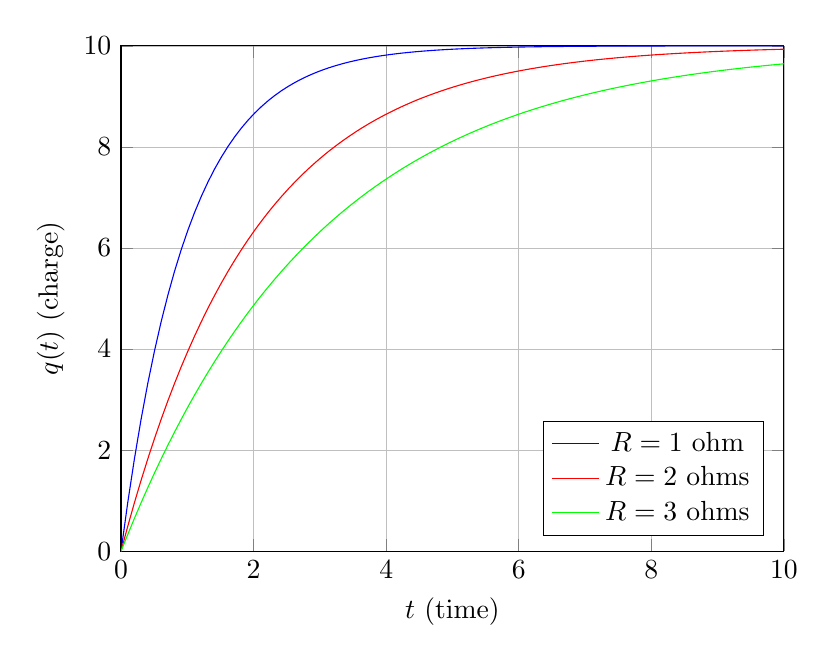
\begin{tikzpicture}
    \begin{axis}[
        xlabel={$t$ (time)},
        ylabel={$q(t)$ (charge)},
        xmin=0, xmax=10,
        ymin=0, ymax=10,
        xtick={0,2,4,6,8,10},
        ytick={0,2,4,6,8,10},
        legend pos=south east,
        grid=both,
        grid style={line width=.1pt, draw=gray!10},
        major grid style={line width=.2pt,draw=gray!50},
        width=10cm,
        height=8cm
    ]
    
    \addplot[
        domain=0:10,
        samples=100,
        color=blue,
        ]
        {10*(1 - exp(-x))};
    \addlegendentry{$R = 1$ ohm}
    
    \addplot[
        domain=0:10,
        samples=100,
        color=red,
        ]
        {10*(1 - exp(-x/2))};
    \addlegendentry{$R = 2$ ohms}
    
    \addplot[
        domain=0:10,
        samples=100,
        color=green,
        ]
        {10*(1 - exp(-x/3))};
    \addlegendentry{$R = 3$ ohms}
    
    \end{axis}
    \end{tikzpicture}

\subsection{Convergence Analysis}

To find the corresponding sequence \( q_{\text{max},n} \) for the maximum charge of the capacitor as a function of \( R_n = nR \), we need to consider the charging curve \( q(t) \) for each \( R_n \) and find the maximum value of \( q(t) \).

From our previous analysis, we know that the charge on the capacitor as a function of time \( t \) for a given \( R \) is given by:

\[ q(t) = CV(1 - e^{-\frac{t}{RC}}) \]

For \( R_n = nR \), the charge function becomes:

\[ q_n(t) = CV(1 - e^{-\frac{t}{nRC}}) \]

To find the maximum charge, we need to find the maximum value of \( q_n(t) \). This occurs when \( e^{-\frac{t}{nRC}} = 0 \), which happens when \( \frac{t}{nRC} = \infty \), or equivalently when \( t = \infty \). Therefore, the maximum charge \( q_{\text{max},n} \) occurs as \( t \) approaches infinity, which is:

\[ q_{\text{max},n} = CV \]

This implies that the maximum charge of the capacitor for each \( R_n \) is independent of \( R_n \), and it is solely determined by the initial voltage \( V \) and capacitance \( C \). Therefore, the sequence \( q_{\text{max},n} \) is a constant sequence, and it converges to the maximum charge \( q_{\text{max}} = CV \) as \( n \) approaches infinity.

Regarding the convergence of the infinite series \( q_{\text{max},n} \), since it is a constant sequence, the series trivially converges to \( q_{\text{max}} = CV \) which means \textbf{sequence is convergent}. There's no need to investigate convergence properties further as the sequence is constant. \textbf{Series is divergent} because the terms do not approach zero and infinite sum tends to infinity.



	\chapter{Conclusion}

Through this project, we learned how capacitors work, how to design one and how to use one in a circuit. We also learned how to measure the capacitance of a capacitor without using a DMM. This project helped us to get hands-on experience with capacitors, oscilloscopes, signal generators and understand their behavior in circuits. The results that we obtained from the experiments were consistent with our theoretical predictions. 

\section{Key Takeaways}
\begin{itemize}
    \item Capacitors store energy in the form of an electric field.
    \item In order to find capacitance, we can use square waves and measure the time taken to charge and discharge the capacitor.
    \item Feeding a triangular wave to a capacitor makes a low-pass filter.
    \item Charge stored in a capacitor is directly proportional to the voltage across it and it does not depend on the resistance in the circuit.
\end{itemize}


	\newpage
	\thispagestyle{plain}
	\printbibliography{}
\end{document}
